% \textcite{} \parencite{}
\documentclass[12pt]{turabian-researchpaper}
\usepackage{turabian-formatting}
\usepackage[american]{babel}
\usepackage{csquotes}
\usepackage{setspace}
\usepackage{quoting}
\usepackage[style=apa]{biblatex}
\DeclareLanguageMapping{american}{american-apa}
\addbibresource{synthesis.bib}
\newcommand{\itab}[1]{\hspace{0em}\rlap{#1}}
\newcommand{\tab}[1]{\hspace{.1\textwidth}\rlap{#1}}
\hyphenation{pho-ne-ti-cal-ly}
\raggedbottom
\usepackage{footnote}
\usepackage{lineno}
\renewcommand\linenumberfont{\normalfont}
\makesavenoteenv{tabular}
\makesavenoteenv{table}
\usepackage{array}
\newcolumntype{L}[1]{>{\raggedright\let\newline\\\arraybackslash}p{#1}}
\newcolumntype{R}[1]{>{\raggedleft\let\newline\\\arraybackslash}p{#1}}
\newcolumntype{C}[1]{>{\centering\let\newline\\\arraybackslash}m{#1}}
\usepackage{titling}
\usepackage{courier}
\usepackage{setspace}
\usepackage{graphicx}
\usepackage{pdflscape}
\usepackage{indentfirst}
\usepackage{hyperref}
\usepackage{enumitem}
\usepackage{tikz}
\usetikzlibrary{intersections}
\usepackage{multirow}
\usepackage{array}
\usetikzlibrary{arrows}
\usepackage{gb4e}
\newcommand{\HRule}{\rule{\linewidth}{0.5mm}}

\title{\textit{Interrogating Person Reference \\ as a Marker of Conversational Genres
}}
\author{Irina Wagner\\ \\ Synthesis paper \\ Committee: \\ Dr. Andrew Cowell (chair), \\ Dr. Barbara Fox, \\ Dr. Kira Hall}

\date{\today}
\begin{document}
\begin{titlingpage}
\setlength{\droptitle}{80pt}

\maketitle
\setwordcount

\end{titlingpage}

 
\doublespacing
\indent

\section{Introduction}
Anecdote: why genre?

``The most important form of art is cinema,'' - wrote Vladimir Lenin suggesting that this form of mass communication would be the most effective for the use of communist propaganda. Indeed, our society is constantly looking for new genres to effectively communicate particular ideas, accomplish particular social actions, and frame social practice. Genres, in a sense, act as schema, or carcass, on which one can draw a full picture with all of its references to the common sense and previous discourse, and at the same time expect a very special type of response from the audience. In other words, genre, at least in arts and literary arts, embodies an effective practice of communication.

Similarly, when talking to people, we tend to use already developed schemes to accomplish particular needs. These schemes organize and structure conversation by the means of exploiting particular linguistic varieties and devices. In this paper, I explore the connections  between person reference in interaction and interaction as a continuum of conversational genres. Previous research deals in a great way with the meaning and use of person reference, however, studies examining the macro structure of interaction seem to engage with smaller categories such as speech events and acts. Here, I propose that the category of conversational genre can be employed to talk about the organization of an interaction with regards to its efficacy in accomplishing particular social goals. On the example of the data from conversations between fluent Arapaho speakers, I demonstrate that the difference in talking about other people can frame the different conversational genres which are used to accomplish particular social goals and provide commentary on the established social practice.

 Concerned with the organization of talk, conversation analysis defines and outlines the structure of a conversation down to the most minimal detail \autocite{SSJ1974}. In general, beyond the adjacency pairs and sequences, there seems to be no term encompassing a span of talk: in his investigation of sequence types and coherence, Schegloff refers to ``clumps'' of talk and ``spate'' of conversation \autocite{Schegloff1990}. Importantly, those terms tend to capture the structural features of a conversation. With regards to the topic of an interaction, as Schegloff notes, the thematic coherence is also achieved by consistent reliance on the sequential organization of a conversation. Meanwhile, other disciplines studying text productively use the concept of genre to delineate the differences in structure, theme, and reception of a text. Here I propose a concept of conversational genres as an effective analytical tool for the linguistic and socio-cultural investigation of naturally occurring conversations, and I demonstrate the category of person reference as an indicator of such genres.

Theories of genre dominate in the literary studies but have also been adopted in linguistic anthropology where genre allows to account not only for the organization of speech acts, styles or events, but also trace their meaning in social practice through the understanding of intertextuality (Briggs \& Bauman, 1992). Being produced and reproduced, certain genre forms may have specific effects in the speech community by triggering the available ideologies and relating them to the previous discourse (Bakhtin 1986). So narrative genres in particular, Hyv\''arinen (2015, p. 181) suggests, ``function as frames of orientation [sic] for the language users themselves within certain social practices.'' In other words, the main advantage of employing genre in analysis is the ability not only to categorize text or performance, but also observe their meaning and reception by a speech community. 

Similarly, my proposal of conversational genres focuses on the link between the text and structure of face-to-face talk and the meaning it forces onto the speakers and their speech community. While such CA concepts as sequence type and speech action indirectly respond to the issues of generic classification and social effect, they do not fully capture multi-unit sequences which create and maintain important social discourses. Relying on the previous work in genre studies, I define conversational genre as a continuum of idealized conventions of single or multi-unit conversational sequences which share similar organizational structure, style, and register, evoke similar response from the recipients, and are subject to interpretation in the moment of speaking in connection with any previous discourses and ideologies.  This definition provides three distinct gravitational poles for conducting further analysis: a) by suggesting that the conversational genres are not strictly categorical, this approach adopts the view of emergent conversation; b) it connects the conversation to the sociocultural realm which is not achieved by any other analytical tools of CA; and c) it incorporates the issue of intertextuality in the understanding of the message and the expected response. Importantly, proposing that conversational genres form a continuum emphasizes the fluidity of conversations and foregrounds the negotiations done by the interlocutors at the moment of speaking. It is my hypothesis that while conversational genres may have some distinct features, speakers are free to modify them in the progression of talk to fit their needs. 
Registers and genres are reported to have an effect on the reference terms due to their access to previous information and establishment of certain connections between the speaker, addressee, and the referent (Clark \& Wilkes-Gibbs, 1986; Harkness, 2015). Previous studies in ethnography of communication and discourse analysis pay close attention to registers and genres, attending to particular linguistic repertoires and features as defining. 

For example, reported speech is often cited to distinguish between narrative and turn-by-turn talk (Rühlemann, 2013; Tannen, 2010). Tannen (2010) suggests that the use of reported speech, or constructed dialog, in written and spoken registers allows speakers to organize and structure their interactions and narratives. They also add a dramatic effect to the narration, causing immediacy of the telling. Similarly, Ruhlemann (2013) explores the pathos of the constructed dialogue and quotations as contributing to the boundaries of embedded discourse (120): he argues that through reported speech speakers can intertwine perspectives and easily navigate between them. Such discourse presentation is possible by using the linguistic feature of quotation and paralinguistic feature of silence to frame and organize the interaction. These features establish boundaries of discourse that allow the recipients to comprehend the perspectives of the narrator and the invoked characters.

Similarly, previous studies in ethnography of communication also note the influence of registers and linguistic repertoires on the discourse genre and the social practice activated by it. So Hanks (1987) in his study of the early colonial documents of Maya in Mexico, draws the connection between the style used in the documents and the authority they were appealing to. In his analysis, Hanks suggests that the Mayan authors intentionally mixed registers and used ambiguous time references to establish the discourse genre that is more appealing to the colonial audience and that reinforces Mayan authority. With this, Hanks argues, different discourse genres employed in the official documents served particular social practice, engaging with the linguistic repertoires of both the authors and the audience. The purpose of my study is to investigate if the same can be said about conversational genres.

Overall, the organization of interaction has not been widely studied with respect to different genres and their boundaries. Yet, it has been established that certain linguistic features affect the genre and its meaning, which at their turn modify the social work and practice accomplishable by the discourse. Although there is no previous research indicating that person reference terminology can be one of the linguistic variants influencing genre, as a feature so tightly connected with cultural and social relations, it is my hypothesis that it is also an organizing feature of interaction.


\section{Conversational Genre (about 10pages)}
%I.	Conversational genre is an important analytical tool for the discussion of face-to-face interactions, endangered languages, and social discourse.
This study proposes a concept of conversational genre as an important analytical tool for the discussion of face-to-face interactions. The main goal of this concept is not only to introduce smaller chunks of conversational discourse for the analysis, but also interrogate them as necessary for deriving the social meaning of the full interaction. Because the conversational genres express the cultural rationale for structuring the talk and engaging in the sociocultural commentary of ideology and practice, it is argued that they are defined by culture and society itself and mimic the goals of the speech community. 

Before diving into the issue of conversational genre, it is important to clarify some of the theoretical concepts used in this study. While the studies on genres are numerous, in discourse analysis in particular they often conflate the differences between text types, genres, registers, and modes into one. Meanwhile, the current study distinguishes between them as the major components making up one another. The proposed hierarchy in these definitions evolves from other works and wishes to explicate the fluidity of discourse and its inherent components. Here, I will mainly focus on the concept of genre since it is central to my research, however, I also wish to present the main points of divergence with the other mentioned elements of discourse. 

\subsection{What is genre}
Theories of genre dominate in the literary studies but have also been adopted in a range of social sciences and in humanities. Categorization of text or performance, approaches its analysis from two different perspectives simultaneously. On the one hand, genres imply internal structural similarities and differences. So, verse in poetry characterizes the poetic organization of the text. On the other hand, genre is also a functional categorization: a particular genre is often associated with the content and context of its text as well as the expected effect on the audience. Nonetheless, this concept is not particularly favored in linguistics due to its ambiguity with other terms identifying linguistic variation(?). Drawing from different approaches on genre in linguistic anthropology and discourse analysis, this section offers to accentuate the connection between genre and social practice \parencite{hanks1987}.  

In linguistics, the focus on the aspects of language beyond text(?) conflates genre with speech events and register, which prompted \textcite{swales1990} to report that linguistics generally finds genre ``indigestible'' (p. 41). So, \textcite{hymes1974} notes this conceptual similarity but argues that genres and speech events are different analytical tools: while he restricts speech events to the activities governed by rules for the use of speech, the concept of genre he associates with types of speech sharing similar structures but invoked at various situations. In his understanding, genre lacks functional component and texts and performances of same genre can be used with the same effect in different situations (or vice versa?). As \textcite{swales1990} notices, this approach would mean that when a sermon is given outside of a funeral for satiric or political purposes, it remains to be a sermon with all of its effects and meanings. Meanwhile, following \textcite{bakhtin1986} and his rhetoric on genre, one can notice that the lack of the functional component in such a definition (whose, Bakhtin's?) also disregards the conventionalism and intertextuality as the essential features of this concept (intertextuality is the essential feature of genre?). By emphasizing the functions and conditions of speech and utterance, he suggests that genres appear in response to them, differentiating self (?) from style and grammar.  

Similarly, the functional distinction seems to be in the center of(a major aspect of) confusing register and genre. \textcite[p. 191]{biber2012} defines register as ``text varieties of a language associated with a particular situation of use,'' also suggesting that register corresponds with the differences in linguistic features according to the desired function of text. In order to differentiate it from genre, Biber suggests that genre analysis looks ``beyond the sentence'' unlike the studies in the register. Furthermore, he proposes also to distinguish the functional and conventional functions of genre: since both register and genre are defined as language variations dependent on the accomplishment of a particular effect, the main difference between them is that of a conventional use of genre. In other words, Biber suggests that linguistic variation according to genre is socially expected to conform to particular rules of language use rather than distinct situational contexts (p. 193). [perhaps you should give some examples of proposed linguistic genres to clarify the discussion]

Following the ``Hallidayean'' approach to genre, \textcite{swales1990} further disambiguates this distinction, stating that register and genre are on different levels of analysis. Register is described as a tripartite system in which each part (field, tenor, mode) responds to different level of text management (correspondingly: ideas, personal relations, and discourse). Importantly, the realization of the text management on each level can only be accomplished by language. Consequently, genre is proposed to be ``underlying to register'' -- a level on which things get done \parencite[p. 40]{swales1990}. Thus, the relationship between genre and register is complementary, each of them is chosen independently in order to achieve the predetermined social goals.
The possibility to find common conventional elements in genre means that no discourse or text is unique(?). By following the socially-expected norms, authors are able to create content that receives expected acceptance. So, narrative genres in particular, \textcite[p. 181]{hyvarinen2015} suggests, ``function as frames of orientation for the language users themselves within certain social practices.''OK In other words, the main advantage of employing genre in analysis is the ability not only to categorize text or performance, but also observe their meaning and reception by a speech community.OK Ultimately, use of a particular genre in speech leads to creating and maintaining social practice by its employment of intertextuality \parencite{briggs1992} and iterdiscursivity \parencite{wortham2015}. Intertextuality can be defined as a structural principle of textuality that remains constant or recognizable across speech events \parencite{wortham2015}. Being produced and reproduced, distinguishing attributes of text may have specific effects in the speech community by triggering the available ideologies and relating them to the previous discourse \parencite{bakhtin1986}. Interdiscursivity specifies how ways of talking can establish chains of speech events, and eventually become associated with certain social types and evaluations creating the trajectories of accomplishing social processes \parencite{agha2003}. Having the intertextual knowledge, audience is able to produce the appropriate reaction to text or a performance, which can be either realized in action, a verbal response, or even rejected.OK So, manipulations of genre are available not only to the authors, who can mix different ones and change the expectations of a reaction for the effects of humor, for example, but also to the audience who may not recognize features of intertextuality and reject the text \parencite{bax2011}. Importantly, the expectation of a reaction indicates the field of possibilities based on the previous talk. In other words, every speech or utterance in the Bakhtinian view is ``linked'' to other ones that have come before it either verbally or orally \parencite[p. 69]{bakhtin1986}. 

Furthermore, in connecting genre to social practice, \textcite{hanks1987} insists that genre(s) actually forms the linguistic habitus of a speech community.OK In particular, he notes that genres cannot persist without the community who understands its conventions, intertextuality, and social meaning, which allows them to be recognized as the core of social practice.OK As an action within a community of practice, genre is conditioned by a set of symbolic characteristics forming a mental schema shared by the representatives of the community. Thus, Hanks concludes, genres like any other schema exists prior to any event of practice, organizing the linguistic \textit{habitus} and yet prone to change and innovation with the changes in the society.

The variations in text and commonality in genre categories indicate that the two of them are different concepts of presentation. Text, being determined by registers and styles of speech, is a concrete product, whereas genre is only ideational because it can only outline or frame the main concepts of text depending on the context and the audience \parencite{bax2011}.OK  The convenience of genre is expressed by its classificatory functions of text and in its overwhelming applicability to different types of speech events. Genre ultimately allows to distinguish similar patterns in structure, expectations, and presentation of text, and categorize texts with similar features together.OK The complexity of text, however, shows that genre categorization is not as unequivocal as it appears to be because of the fuzzy boundaries of textual categories and the possibilities of genre mixing. The capability of authors and speakers to mold their text in response to a varieties of factors makes hybridity of genres inevitable and complicates proper categorization of texts \parencite{bax2011}.OK On the other hand, \textcite{bakhtin1986} sees genre hybridity, or as he calls it ``flexibility,'' as an inherent feature of communication. The creativity of authors or speakers is essential in communication, which leads to pure impossibility of a comprehensive list of all of the speech genre. At the same time, he notes, that the better knowledge of genre opens up better possibilities in more ways of using them for social communication.

A step toward creating a list of genre lays in the understanding of the varieties, conventions, and purposes of communication. So, the idea of discourse modes as the possible varieties of these processes describes distinct possibilities of using written and oral text for the purposes of achieving different contextual effects. \textcite[p. 54]{bax2011} explains that discourse modes are different from genre in a more abstract, pre-existing sense, by defining the possibilities of using the language rather than simply extracting its values.(?) Depending on the approach to discourse modes, they are usually recognized by what they are attempting to do: narrate, describe, and argue.OK An additional mode that is often included in this list is conversation, or dialog, which is also often conceived to be the essential abstract form of human communication \parencite{bakhtin1986, bax2011}. As Bax explains it, genre can implement several discourse modes, so for example, in a novel one can find both conversations and narratives, neither of which change the structure or function of the novel genre.OK 

The essentialism of the narrative and conversation (interaction, or dialog) indicates their accessibility and availability.(?) In fact, when trying to outline discourse modes, \textcite{georgakopolou2000} simply distinguish between narrative and non-narrative discourse. The simplicity of such an approach may not account for the variation in arguments and interaction, yet, it emphasizes the primacy of narrative in the everyday communication. Narratives fulfill multiple functions in our social activities, including socialization, processing of events, organization of the community, and ensuring the cohesion of the culture \parencite{georgakopolou2000}. The term ``narrative'' is being used in its broadest sense as a rhetorical mode that recounts or represents ``some temporally instantaneous event'' (p. 123). The main defining feature of this discourse mode is its referentiality: informed by the context of an interaction, narrative attempts to reconstruct the reality while non-narrative, or conversation, aims to verify or validate it. So, one thing that non-narrative modes, such as conversations, have in common is their tendency to establish truth by the means of different interactional techniques, such as interrogation, evaluation, argument, etc. While these techniques are also available in a narrative, they cannot be used without reproducing a durative event in the heights of the story. 

Textually, both of the discourse modes differ in the pattern of their structures. \textcite{bakhtin1986} proclaims dialog the most basic form of communication for(due to) the simplicity of its structure: turn-taking in conversation, according to him, creates clear-cut boundaries between utterances while also maintaining the contextual relationship between them. So, speakers are aware that after a question in a conversation, the answer follows.. Such relations are not possible elsewhere in  language, neither between words, nor sentences.(really?) However, in  narrative, a different structure emerges, indicating a specific pattern characteristic to this discourse mode. Because of its attempt to reproduce durative events in somewhat time-related manner, narrative discourse tends to have an internal time sequence organization that can be narrowed to orientation, complication and resolution \parencite{labov1967}. Additionally, non-narrative discourse uses intonation and paragraphing(?) for its organization(do you really want to claim that non-narrative – i.e. conversational – discourse relies on only intonation for organization? And the claim for paragraphing seems completely out of place when talking about discourse), while narratives rely primarily on the features of its content (time, place, characters) and rhythmic units, such as verse and stanza (again, seems like not the best general description of the organization of narrative, which relies primarily on temporal sequencing devices such as ‘next, so then, and’ etc, (in English) and inferred or explicit causal connectors) \parencite{georgakopoulou2000}. With these considerations in mind, one would also expect more fine-grained distinctions in the way each of these modes uses language: in particular, referring to(with reference to?) style and register. 
Having outlined the main concepts of each of these two discourse modes, I must also note that these modes are not exclusive, since conversational narrative is also a possibility that comes with a variety of its own structural, contextual and referential features. \textcite{norrick2000} indicates that sequentiality of time, while often relevant, can be omitted in the narrative to appeal to a particular point. Moreover, the boundaries of a narrative are much less distinctive in a conversation because the narrative pattern may not follow the established conventional route(?) and may not have distinctive boundaries even in the beginning and the end. Yet, previous research on conversational narrative shows it to be a particular type of discourse differentiated from other modes by the types of register it employs (among many other features, of which register seems to be among the more minor differences).

In general, when talking about discourse, it seems most appropriate to differentiate it into separate [levels (units?) of meaning(?)] based on the functions and structure of its parts. Here, I discussed [where in the discourse system lays genre how the concept of genre can be understood in relation to the broader concept of discourse], and based on the previous studies I suggest that it takes an intermediate position between discourse modes and registers. Discourse modes, unlike genre, outline only the contextual and textual features of the text which normally refer to the general structure and specific devices that it uses. Unlike genre, rhetorical modes are not patterned by agreed-upon conventions and do not influence social practice. On the opposite, they merely function as a frame of text presentation and genre may combine them. Registers, on the other hand, function as minimalistic representations of linguistic variation. By employing certain linguistic repertoires and varieties depending on the context, registers add metalinguistic information to the text. Genres are said to be in the intermediate level of text production as they combine the information provided by the registers and apply it within a particular discourse mode. Speakers know how to alternate structural composition of text in order to achieve a particular response from the audience. Conceptualizing genres as conventional mental schemes, this approach accentuates the role of society in the production and reproduction of genre. In a sense, genres are presented here as ``socially endorsed'' as though only the speech community can agree upon their functions and features, while individual speakers have no control over them \parencite[p. 60]{bax2011}.
  
So, while defining ``genre,'' some of its features must be especially emphasized in order to distinguish it from other linguistic concepts such as speech event, register, style, and mode. What comes from the discussion above is that key aspects of genre are its functionality and conventionalism. So genres, unlike other categories, perform particular discursive functions and are defined by socially accepted conventions on the presentation of the text and the proper reaction to it. Because of this strong connection between genres, conventions, and speech community, genres are argued to form part of the linguistic \textit{habitus} of a speech community. Genres are also defined by their particular structures, which conform to the previously known productions of text. In their construction, genres can use a variety of linguistic devices in order to correspond with the appropriate features[expectations for production and reception?], such as particular registers, styles of speaking, and varying grammatical features. At the same time, correlations of registers and genres can also indicate the successful comprehension and effect of text on  social practice. With that, it is important to highlight that the connection between genre, registers, and styles of speaking is bilateral[often mutually reinforcing?] and multi-leveled[complex?]. 

\subsection{Conversational Genres}
B.	This research fills the gap of using the approach of genres in conversation analysis to connect it with the linguistic variation in the discourse and creation and support of important social themes/discourses.

1.	Definition of CG.

1.	Bridging the structural-functional gap: genre is multi-faceted, and leveled. We can’t talk about distinct genres, but we need to understand their continuum and their connection. 

2.	Possibility of employing a nested categorization: structure on one end/level --> function on another level.

3.	The major macro-genre distinction: narrative g. and non-narrative g. 

4.	Examples of CG from Data?

\section{Person Reference}
The feature of person reference is a well-researched topic in conversation analysis. Besides being interesting from the point of view of membership categorization, person reference is also a useful indicator of internal structure, recognitionality, and semantic frameworks available in the conversations. Although most of the studies in person reference have been performed on English, some recent researches also looked at referring practices in lesser studied languages, expanding our view on the principles of referentiality. In general, there seems to be an agreement between the researchers that person reference have both structural and cultural principles behind their choice. Here, I would like to discuss the logic for the principles in the current research. I aim to demonstrate that beyond their grammatical, structural, categorizing, and referential principles, terms of person reference also play key role in identification and construction of the conversational genres.

Choice of person reference terms depends on the conversational structure as well as familiarity of the interlocutors with the referent. The research on this subject demonstrates several significant attempts to describe the principles of that choice which can be roughly narrowed down to structural, cultural, and grammatical principles. Importantly, while these principles are not reductive, they have never been put together to demonstrate referentiality, rather they appear as competing theories. Meanwhile, treating these principles as separate and reductive would essentialize referential practice. 

\subsection{Structural Premises}

The two major principles underlying the choice of person reference terms are described in the initial study by \textcite{sacks1979}. According to them, a successful term of person reference should be short but at the same time semantically loaded to be recognized from the first attempt at pronouncing it (p. 24):
\begin{enumerate}
\item ``On occasions when reference is to be done, it should be preferredly be done with a single reference form.''
\item ``If they are possible, prefer recognitionals.''
\end{enumerate}
Having numbered these principles, Sacks and Schegloff, nonetheless, emphasize that recognitionality is most important and must be achieved first. They argue that ignoring the principle of recognition may cause extra work of disambiguation to the speakers and become counterproductive in conversations. In general, recognitionality or recognizability implies that in any given moment in conversation the speaker must be aware of the knowledge of the referent by the addressee. This statement makes recognitionality a feature of recipient design that can structure conversation by implications of shared knowledge or by requiring additional clarifications and disambiguations. 

The term ``recognitional'' is a vague one and can be better described by the presupposition of inherent knowledge of speakers. While it is often equated to ``identifiable,'' the two have different properties. ``Identifiable'' is a term applicable to objects and subjects that are uniquely distinguished from one another \parencite{clark1986, chafe1976}. ``Recognitional,'' however, refers not just to the identification of the object, but also connotes the shared mutual knowledge of the object’s properties \parencite{clark1986, defornel1987, sacks1979}. As \textcite{chafe1976} notes, for something to be recognitional, it needs to be semantically available in the domain of talk. So, for a speaker to use a reference to a person not previously brought up in the conversation, there needs to be substantial semantic and pragmatic background. An example often cited from \textcite{schegloff2007} is the anaphoric use of the third person singular pronoun when speaking about John F. Kennedy shortly after his attempted assassination. While ``he'' is an identifiable pronoun, the reference is recognizable because shortly after the event, the tragedy was on the minds of many people in the U.S. and ``he'' was a mutually shared understanding of the President. In sum, recognitionality of a referent is a collaborative achievement: while the speaker must make such a referent identifiable based on the understanding of shared common knowledge, the addressee either must provide information beforehand about the possibility of understanding, or must recognize that reference without needing additional disambiguation.

The principle of recognitionality is tied in with the structural properties of a conversation which can determine the more proper form of reference. In her study of the anaphoric reference, \textcite{fox1987} demonstrates that a speaker would not use a minimal reference term unless that referent has already been introduced and reoccurs in the still open sequential construction. Fox argues that interlocutors track whether the sequence is still closed or open before they choose the appropriate form of person reference, demonstrating the dependence of the reference term on structural organization of the conversation. Employing the concept of ``return pop'' borrowed from natural language processing, Fox explains how the structure of a conversation can be understood and negotiated by the interlocutors. So, a minimal reference term such as a pronoun is not just the indicator of an open sequence, but it can also mark the importance of the closed adjacency pair for the conversation by reintroducing same referent anaphorically. In a sense, the organization of non-story talk is activated by the person reference terms and is also shaped by them.   

Similarly, in a different research \textcite{schegloff1996b} also demonstrates the connection between the forms of person reference and the structure of talk. In order to define preferentiality in the form of reference, he distinguishes between initial and subsequent terms and positions. Schegloff considers locally initial forms such reference terms that identify the referent for the first time (i.e., full noun phrases or names) and locally subsequent forms are the terms of reference that merely point back at the already identified and recognizable referent (i.e., anaphoric devices such as pronouns). As he demonstrates, the coordination of the position of reference in talk and the term of reference has implications on the structure of the conversation. Table (\ref{form-position}) summarizes Schegloff's findings with regards to matching and mismatching the positions and reference forms.

\begin{table}[]
\centering
\caption{Structural features of reference forms and positions according to Schegloff (1996).}
\label{form-position}
\begin{tabular}{l|l|p{2in}} 
& \textbf{Locally Initial Form}                                                                                                                                         & \textbf{Locally Subsequent Form}                                                                                                                             \\
\hline
\\
\multirow{3}{1in}{\textbf{Locally Initial Position}}&  & - availability of the referent to both interlocutors;\\ & {Preferred}                                                                                                                                                              & - indicates continuation of talk;\\ & & - re-opens the sequence.\\
\hline
\multirow{4}{1in}{\textbf{Locally Subsequent Position}} & - indicates sequence boundary;\\ & - shows disagreement;\\& - often a recycled element in the overlap;& {Preferred}                                                                                                                                             \\ & - used to restart a term. 
\end{tabular}
\end{table}

Importantly, while Schegloff notes that mismatch in the position and form is possible, he argues that it is a conscious choice of a speaker who offers more than just a simple reference term. Reference \textit{simpliciter}, as \textcite[p. 1307]{hacohen2006} describe it elsewhere, is the most essential function of a reference term which does ``just referring'' and nothing else. The additional meanings of reference can include negotiation of conversational structure, disagreement, change in a speech act as well as membership categorization of a referent. In outlining the preference for locally initial and subsequent forms and positions, \textcite{schegloff1996b} is precisely referring to these potential functions of a disprefered reference.

When it comes to the potential forms of reference, several have already been mentioned here, such as full noun phrases, names, and pronouns. In general, they can be differentiated into descriptive, neutral, and anaphoric mentions. As it follows from the discussion above, anaphoric mentions are usually the ones that do not require establishment of an identity of the referent, and thus, they most often appear in the subsequent discourse. Neutral reference terms would be names, or somewhat arbitrary terms for referring to people that do not convey any additional meanings of empathy. Descriptive terms, however, go beyond establishing the identity of a referent and introduce membership categorization, stance, affinity, physical presence, linguistic presence, etc. – creating the ``semantic silver lining'' of person reference \parencite[p.132]{defornel1987}. The main difference between reference by name and reference by a descriptive term is that descriptors tend to attend to a property of a referent, also offering a judgment of the person and evaluating that mentioned property. Essentially, descriptive and neutral terms of reference are not interchangeable, and \textcite[p.136]{defornel1987} suggests that they operate based on the third principle of preference for the relevant role: ``choosing the relevant role is at the same time tacitly bringing into play contextually appropriate properties which are linked to the role within a social frame.'' In other words, the choice between name and descriptor relies both on successful recognitionality and the sufficient information conveyed by the term. Since names are empty of property evaluations, they cannot be used in certain speech acts.

In general, names are the preferred first time reference term in English conversations because they offer the most economic reference to a person and yet the most recognizable reference to a person \parencite{downing1996}. As Downing points out, names are a unique reference term category which can only be employed when the speaker is certain of identifiability of the referent. It means that using a name by itself can prove useless either to such interlocutors who do not know the referent by name or to such situations where referent has not yet been ``activated'' (p. 97). In such situations, speakers may use a full proper name or modify it by adding a noun phrase. In addition, speakers are shown to have other devices available to signal uncertainty about identifiability, such as try-markers \parencite{sacks1979}, noun phrases, or even explicitly negotiate the identifiability of a referent. The latter can be done by informing the addressee about such uncertainty before bringing in the proper name reference:

\begin{figure}
\caption{Explicit negotiation of referent's identifiability (Downing 1996, p. 100).}
\label{Downing}
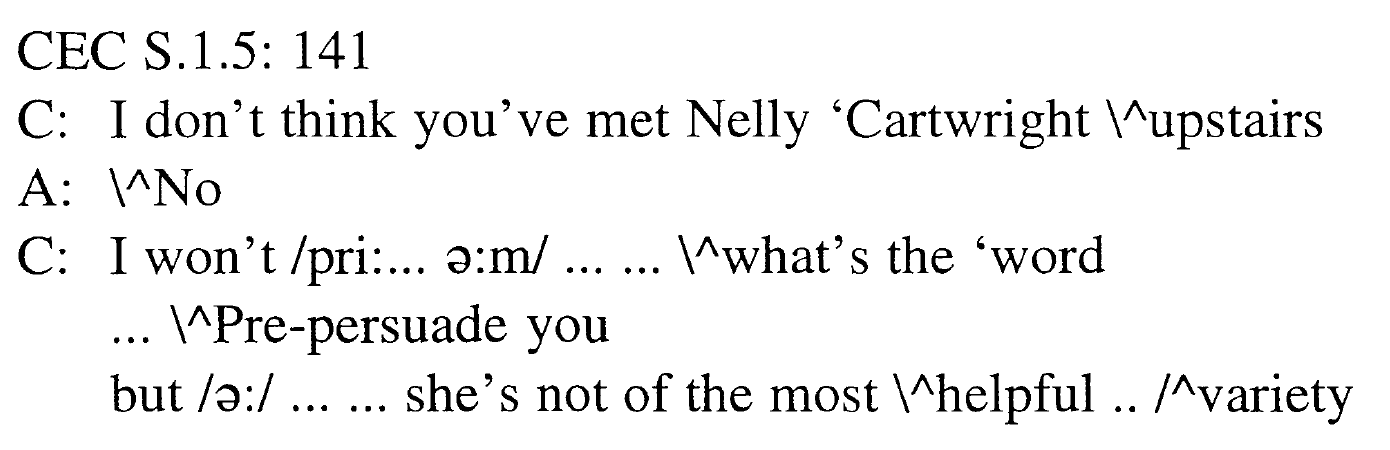
\includegraphics[width=\linewidth]{Downing.png}
\end{figure}

The pre-introduction of the reference term in the first utterance serves to avoid identifiability issues caused by the use of a full name. In general, reference by name is an important linguistic feature as it has a meaning beyond the communicative understanding: using name references not only identifies new referents in a conversation, but also outlines the knowledge boundaries of both interlocutors. In other words, personal names while serve to be the default terms of person referent, are also incredibly useful markers of epistemic stance.
As default reference forms, names serve few pragmatic functions in the conversation. In her study of ``alternative recognitionals,'' \textcite{stivers2007} demonstrates that speakers tend to use these types of reference when accomplishing a particular social action. She argues that some reference forms are a better fit for some speech types because by using such terms, speakers are able to claim a certain degree of familiarity with the referent and even align or misalign with them. So, while names are neutral and can be used across different speech acts and social situations, some references, for example, kinship terms with possessive personal pronouns become especially useful for affiliating with the referent or the speaker depending on the task being accomplished. In the following example Stivers demonstrates how such disaffiliation with the referent can be achieved by placing him in the responsibility domain of the addressee with the second person possessive pronoun:

\begin{figure}[h]
\caption{Example of disaffiliation from the referent (Stivers 2007, p. 80).}
\label{stivers}
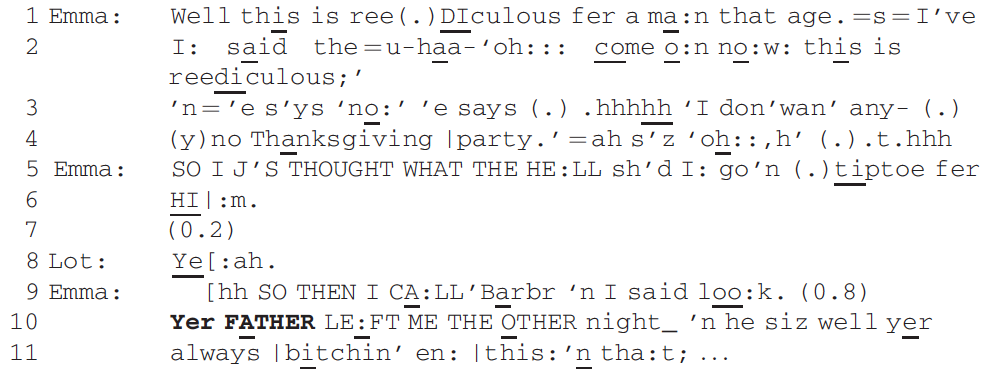
\includegraphics[width=\linewidth]{stivers}
\end{figure}
While a neutral term `dad' is also possible here, Stivers argues that it would have not achieved the same result because it would have not framed the utterance as a complaint. So, the speech act of complaint is intensified by using this alternative recognitional form. In sum, this study suggests that person reference is not just a semantically loaded expression in the conversation, but it is a tool used in conveying social meaning. 

This summary of the research arguing for the structural premises in person reference demonstrates the depth with which this topic has been studied. While all the mentioned works argue for the connection between the form of reference and their relative position in the conversation, it becomes clear that speakers use reference terms beyond referring to manipulate the flow of the conversation and take certain conversational positions. The three principles that have been mentioned thus far, principle of recognition, economy, and role relevance, shape the reference term in accordance to the already available information conveyed by the organization of talk. However, as other research shows, some cultural principles also play a major role in establishing the reference even though they are perceived independent of the conversational structure. 
  
\subsection{Cultural Premises}
Research on person reference in languages other than English also demonstrates that besides these structural principles, culture also determines the types of reference forms that are allowed. Some of such principles recognize the difference in person reference terms that may be more amicable (such as ``mommy'' instead of ``my mother''), that may stem from bilingualism of the speakers (``John'' vs. ``Juan''), that may be defined by avoidance rules, that are differentiated in the community due to multiple names policies, etc. In general, these restrictions can be summarized by the principles of circumspection, introduced by \textcite{levinson2007} and association, introduced by \textcite{brown2007}. Along with the structural principles, they form a system of person reference that is argued to be common across languages yet variable across cultures. In the following pages, I will outline the main ideas behind the cultural preferences and contextualize them in the research on their relative competition in conversations.  

The existence of these two cultural principles reflect constraints on expression of relationships between people in a given community. Circumspection is a response to the rules of avoidance in the community, and association is a response to valorization of kinship. While they are both restricting principles, which means instead of fully identifying the referent they tend to restrict the set of possible referents, they are complementary \parencite{blythe2009}. So, unlike principles of minimization and recognition, circumspection and association do not compete, rather they aid each other in restricting the reference. With regards to their collaboration with the structural principles, the competition between all principles is determined by cultural predispositions. This means that different speech communities prioritize some principles over others in establishing reference, which can only be described in terms of salient features of person identification \parencite{enfield2013a}. 

Avoidance type relationships are said to form the principle of circumspection. This principle prescribes to ``show circumspection by not over-reducing the set of referents explicitly'' \parencite[p. 31]{levinson2007}. This principle suggests limiting the number of the possible referents due to the avoidance or taboo rules common in a specific culture. As Levinson explained, in some of the indigenous Australian cultures, there are taboos associated with the dead that would not allow one to pronounce any lexical item phonetically close to the dead person's name. Or on some occasions one would not want to fully identify the person because it may cause an adversary effect (e.g., punishment for doing something wrong or start an unwanted gossip). Instead speakers would rely on vague hints or general descriptors to establish reference. 

In general, the principle of circumspection can be understood as going against the grain from the principle of recognition outlined by \textcite{sacks1979}. \textcite{levinson2007} clarified, however, that all these principles are applied together and together they optimize the person reference. So, by aligning the types of possible references from the most ambiguous (pronouns) to the most restricted (names), Levinson suggested that each of these principles pulls the choice indicator to different direction in order to find the most appropriate reference term: while the principle of the recognition directs the speaker to use the types of references that are most recognizable, such as kin terms or names, the principles of economy and circumspection pull this choice towards the less recognizable and more ambiguous terms.
\begin{figure}[h]
\caption{The process of competing principles in person reference (Levinson 2007, p. 34).}
\label{chart}
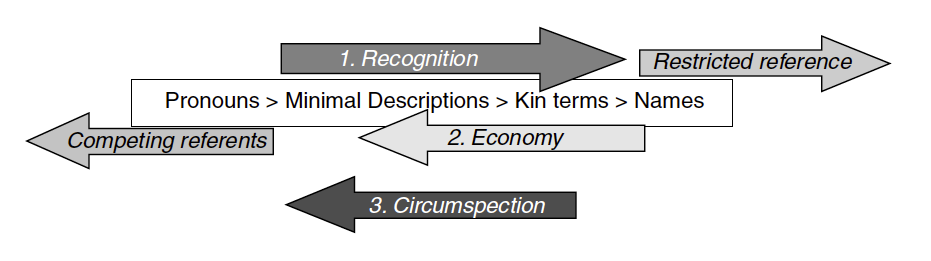
\includegraphics[width=\linewidth]{chart}
\end{figure}
These principles are still not ideal in reference, and Levinson demonstrated it with his analysis of other-initiated repair. So, when a reference term is used but it is still ambiguous the addressee can ask the speaker to clarify it. According to Levinson, due to the principle of circumspection, speakers slowly upgrade a reference term turn-by-turn only if necessary:
\begin{figure}[h]
\caption{Upgrade of reference term in Yélî Dnye due to circumspection principle ambiguity (Levinson, 2007, p. 58).}
\label{levinson}
\includegraphics[width=\linewidth]{Levinson}
\end{figure}
The example in Figure (\ref{levinson}) demonstrates escalation of the person reference term from ``zero'' in the first utterance to a descriptive term due to the other-initiated repair (\textit{n:uu} `who') and later to a name due to subsequent misunderstanding signaled by gaze. So, while the cultural principles of avoidance are followed in avoiding the referent directly, the principle of recognition takes over causing the ambiguity and leading the speaker to clarify the reference. According to Levinson, the principles forming person reference are closely interconnected and their balance is best observed in the default references such as first names in the English-speaking cultures and kin terms in some others.  
In general, the cultural principles determine the default types of person reference, and the deviation from the unmarked has been studied as conveying additional social work. In her study of non-minimal types of reference in Tzeltal, \textcite{brown2007} outlined the default reference practices and ties them with another principle – association: ``associate the referent as closely as possible to the current conversation participants'' (p. 200). Unlike in English, in Tzeltal kin terms are the unmarked or default forms of reference to people in conversations which, Brown argued, causes the formulation of the new principle. So, it is preferred to refer to a person in such a way that would establish the connection between the referent, addressee, and the speaker. If one cannot formulate such a reference term, then it should be done by displaying the kin relation of the referent and the addressee. Although such references may violate the principle of economy, Brown argued that it is more important in that social community to establish the relationship in favor of recognition. 

Studying Yucatec Maya language, \textcite{hanks2007} argued that an appropriate reference is determined by a set of cultural and discourse factors. While the descriptive terms are unmarked in this language, similar to Tzeltal, the kin terms are the default forms of person reference. Yet, the way that one would choose to establish the relationship depends on the type of relationship, associated respect, participation framework in the interaction, and the discourse context of the reference. So, to define a propositus of the kin term, or the point of reference, the speaker essentially needs to decide which social background information is the most relevant to the talk: person reference is a ``construal of person'' \parencite[p. 149]{hanks2007} which in individuating the referent attends to the shared background knowledge of the speaker and the addressee about them. This means that by the construction of a reference term, the speaker also negotiates important matters of the subject's identity, chooses to claim a relation or responsibility to them, and defines the overall social discourse of the talk. The practices described for the Yucatec, and especially the discussion of emotions of respect evoked by kin terms of reference ground the association principle. However, in his discussion of Yucatec person reference, Hanks does not speculate on the social functions of certain names or reference terms, leaving this important issue unattended.

Working with another Mayan language community, \textcite{haviland2007} studied the possible alternatives in reference in Tzotzil. Having found that kin terminology is also the default form of person reference, he argued against \textcite{schegloff1996b} and suggested that reference is never simple, but it is always used to index social relationship – ``referring dupliciter'' (p. 232). The data that he examined perfectly demonstrates that each mention of a person reference tends to create a projection of relationship between the speaker, the hearer, and the addressee. In fact, one of the most important findings of this research foregrounds the principle of association suggesting that it is, perhaps, the most fundamental principle in reference.

The possibility of discerning the meaning from a marked form of reference has been already discussed along with the structural principles. In a study of reference variation in Murriny Patha conversations, \textcite{blythe2009} added that reference introduces meaning both on macro and micro levels of discourse. Besides merely creating references through association, speakers also express their stance towards cultural values, such as clan membership. So by choosing a form that corresponds with the principle of circumspection and association simultaneously, speakers also define their own position towards the cultural prescriptions of avoidance while placing the referent in the recognized network of social connections.

With regards to the meanings invoked by some forms of person reference, in addition to the phenomenon of alternative recognitionals \parencite{stivers2007}, a new concept avoidance recognitionals was introduced to account for the restrictions of references accomplished by the cultural principles \parencite{blythe2009}. Since speakers of the language like the speakers of the mentioned Mayan languages make up a relatively small closed community in Northern Australia roughly any type of identifying construction can be considered recognitional. However, existence of avoidance rules leads to using avoidance recognitionals – the type of ``recognitionals that are used when a referent's name is restricted and ``avoidance'' needs to be performed'' \textcite[p. 213]{blythe2009}. Here, the most frequent types of references are the ones that exploit association by ``triangulating'' the reference -- connecting it both to the speaker and the addressee by the means of kin terms. Blythe advanced Hanks’s \textit{construal of a person} to discern the meaning behind triangulating references according to a particular propositus. In his analysis, self-association allows speakers to claim knowledge and authority of the referent and the events surrounding them by establishing the ``stamp of epistemic authority'' \parencite[p. 231]{blythe2009}. Addressee-associated triangulations, on the other hand, are the forms that simultaneously satisfy association, recognition and specification which secures the recognition of the referent by the addressee allowing speakers to emphasize relevant social networks involved in the constructed relationships. Additionally, research shows that altercentric person reference also establishes epistemic significance by placing the referent into the addressee’s domain of responsibility \parencite{stivers2007}. So, the research shows that the triangular forms of reference using the association are able to not just connect the referent to the addressee or the speaker, but they also provide the ground to comment on the cultural foundations of the community.

The cultural principles driving person reference indicate the great amount of variation possible across languages and communities. The major important feature of these principles shows that reference in conversations has both macro- and micro-interactional meanings. On the small scale, references establish the identity of the person being talked about either by identifying them or by restricting the set of possible people. On the large scale, person references reflect the speaker's stance towards cultural predispositions about social networks. In general, cultural principles while argued to be generally universal, are prioritized differently across languages, with some languages and communities favoring circumspection and others favoring association. Importantly, they never determine the form of reference individually, in that they are only active in combination with structural principles.

\subsection{Intersection of Structure and Culture in reference formation}
The area where both these determining sets of principles have traditionally met is ethnography of communication. In this anthropological approach to description of social and linguistic practices, researchers have been most interested in how text or interaction contributes to creation of social meaning \parencite{hymes1989}. Ethnography of communication is also the sub discipline that with the greatest detail investigated the meanings of kinship terminology and kin relationship in speech as well as performativity of talk. In the following description, I would like to attend to the few important studies that investigated variation in person reference based on the broader meaning it produces. In particular, I will talk about the use of anaphorical mentions in talk, problematizing reference through repair, indexicalities of references, and associated membership categorization. 
As it has been mentioned, anaphorical reference forms do not need to appear in locally subsequent positions \parencite{schegloff1996}. But as \textcite{hanks2007} argued, while their occurrence in anaphorical chains can be traced back to the previous discourse, their occurrence outside of one presupposes background knowledge or prior experience drawing the pragmatic frame of the interaction. In other words, anaphoric mentions outside of the anaphoric chain, or not in the locally subsequent positions, index the relationship between the referred person and the established discourse. Furthermore, to interpret the whole schema employing these indices, one needs to be familiar with both the pragmatic framework and the indices themselves. In other words, the proper understanding and interpretation of reference terms cannot be achieved without understanding the discourse and its sociocultural underpinnings, precisely the area targeted by ethnography of communication.

Thinking of indexicality of reference terms, an important research by \textcite{harkness2015} comes to mind. In his study of different forms of address in a Korean Christian church, Harkness observed not just the connection between the reference term and associated pragmatic framework, but direct correlation between reference and behavior of individuals evoked in it. So, in his study, the members of a Korean Christian church preferred to use kinship terminology (especially such terms that evoke relationship of siblings) when addressing each other. Besides establishing family-like relationships between unrelated individuals, this also sanctioned the behavior seen only in kin folk. In its most basic interpretation of Harkness, terms of reference contribute to the enregisterment models of kin relationship which consequently license particular types of behavior. What is important from this study is that relationship, when channeled in interaction, simultaneously comments on the alignment and affect of the individuals involved in it. 

The principle of association, discussed earlier, can now be re-interpreted from the point of view of indexicality. If kin terminology directly signifies the relationship between the speaker and/or the addressee and the referent, the evoked relationship also serves to validate certain types of behavior, or discourse. Secondarily, the evoked relationship also indicates the speaker's content with the culture that outlines this type of behavior and discourse. So, when using the principle of association, speakers not only create the connection with their addressee or the referent, but also open a discourse of proper relationship models between these people. From the point of view of ethnography of communication, studying the occurrence of kinship terms as forms of reference would provide insights on the saliency of kin relationship between people, and the re-creation of kin network by the means of social interaction.

Having said that recognition is one of the most important features of reference, it needs to be mentioned that studies of failed recognition and subsequent repair are crucial to the understanding of reference. As \textcite{sidnell2008} demonstrated, CA methodology can be especially helpful for sociocultural linguists in examining and interpreting social organization through the lens of repair organization. So, using the principle of association can guide speakers to form a referent, the construed identity of a referent is never set and remains a subject to negotiation. \textcite{blythe2009} argued that the polarity of association can be changed and challenged in interaction to problematize both the reference and the association. A request to repair the reference allows interlocutors to agree on the most relevant form to establish the discourse and re-imagine the pragmatic framework of talk-in-interaction. Yet, other-initiated repair is a potentially face-threatening act towards the speaker, and when used adds a new social meaning to the utterance. The rules of politeness determine when and among who such repair is possible, as politeness in repair is directly associated with the responsibility for the trouble \parencite{sidnell2008}. Thus, construal of person is not finished until both interlocutors have agreed on the referential, functional, and social meaning of the reference.

\section{Person Reference as an index of Conversational Genre}
I.	Conversational genres can be distinguished by the type of reference being used in certain (FPP/first mention) structural contexts. The easiest distinction that they offer is that of narrative vs. non-narrative conversational formats.
\subsection{Narrative}
A.	Narratives in conversations and their co-occurrence with person reference types.
1.	[Detail of the information]
1.	[Detail of the information]
\subsection{Non-Narrative}
A.	Non-narrative conversations. 
1.	[Detail of the information]
2.	[Detail of the information]

\section{Conclusion}

\printbibliography

\end{document}